\section{Applications}
\label{ch:app}

This chapter we first introduces a possible application of our proposed model
and how it could benefit user, the proposed design of the application including frontend, backend architecture as well as database that mostly suitable for the data collection.
Then we formalize and discusse the possibility and benefits as a standard Web API for developers.

\subsection{Client-side Browser Plugin}
\label{sec:plugin}

We developed a client-side browser plugin is an illustration of our model applications.
The plugin proactively serves its user, and providing proactive notification
based on the historical actions in a session.



\begin{figure}[H]
    \centering
    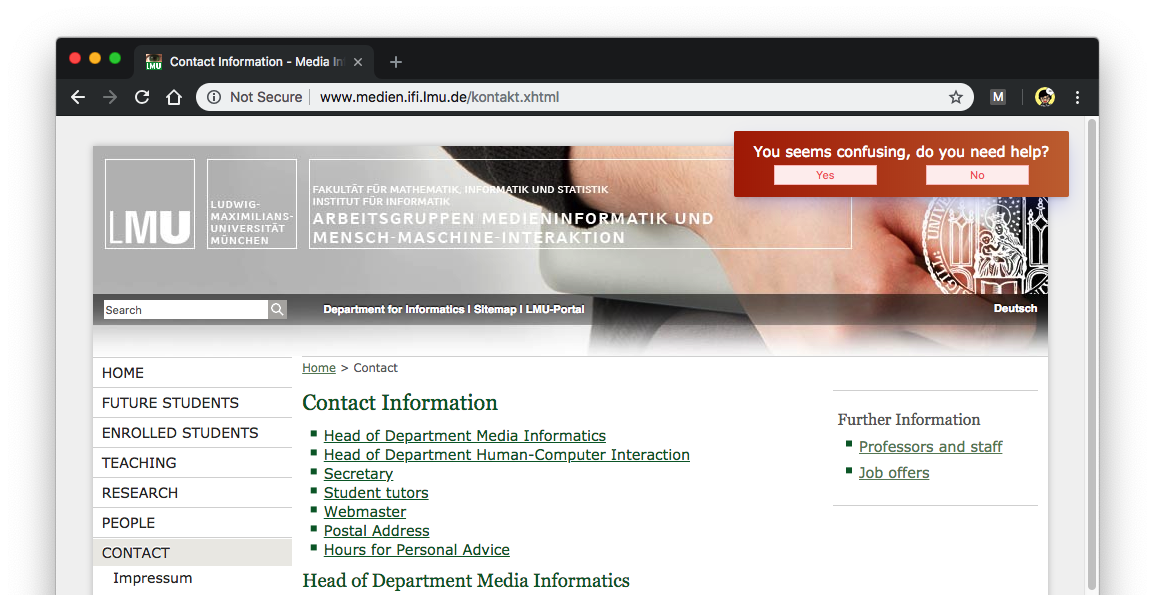
\includegraphics[width=0.7\textwidth]{figures/proactive-noti}
    \caption{TODO:}
    \label{fig:proactive-noti}
\end{figure}


\begin{figure}[H]
    \centering
    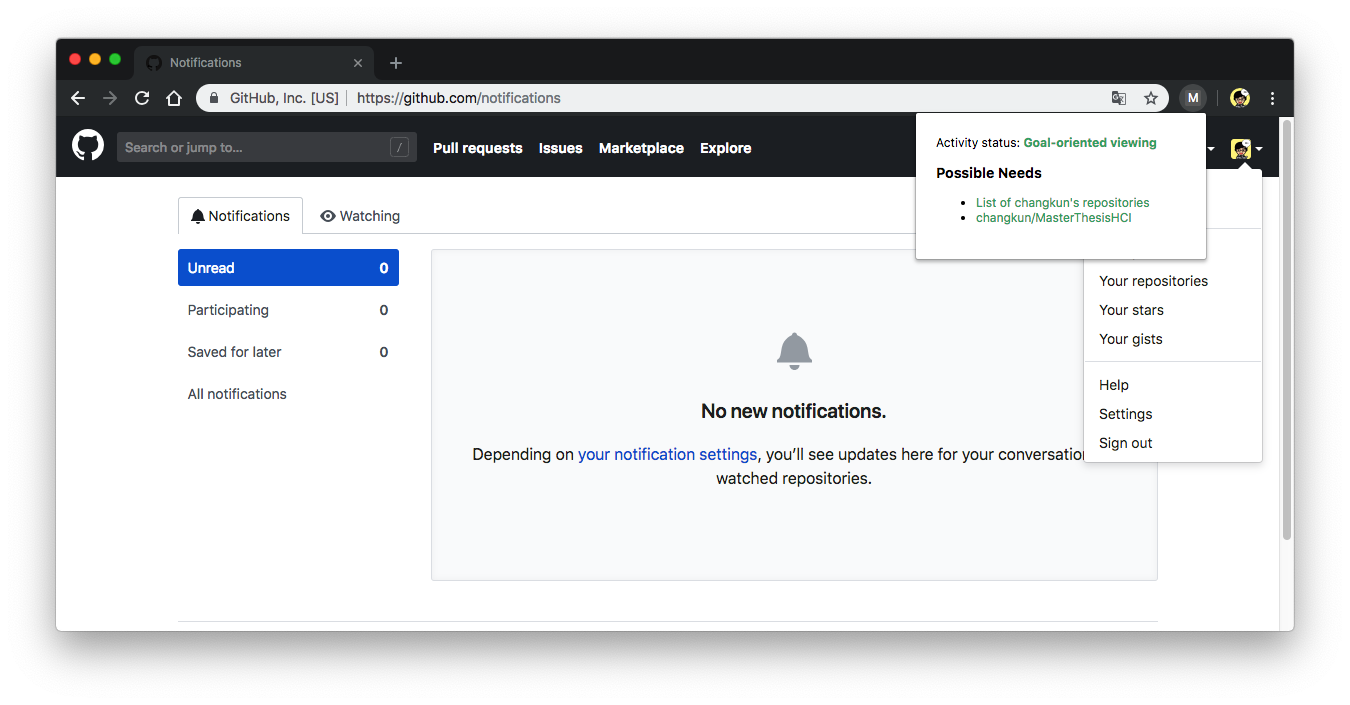
\includegraphics[width=0.7\textwidth]{figures/plugin-predicting-result}
    \caption{TODO:}
    \label{fig:plugin-predict}
\end{figure}

\begin{figure}[H]
    \centering
    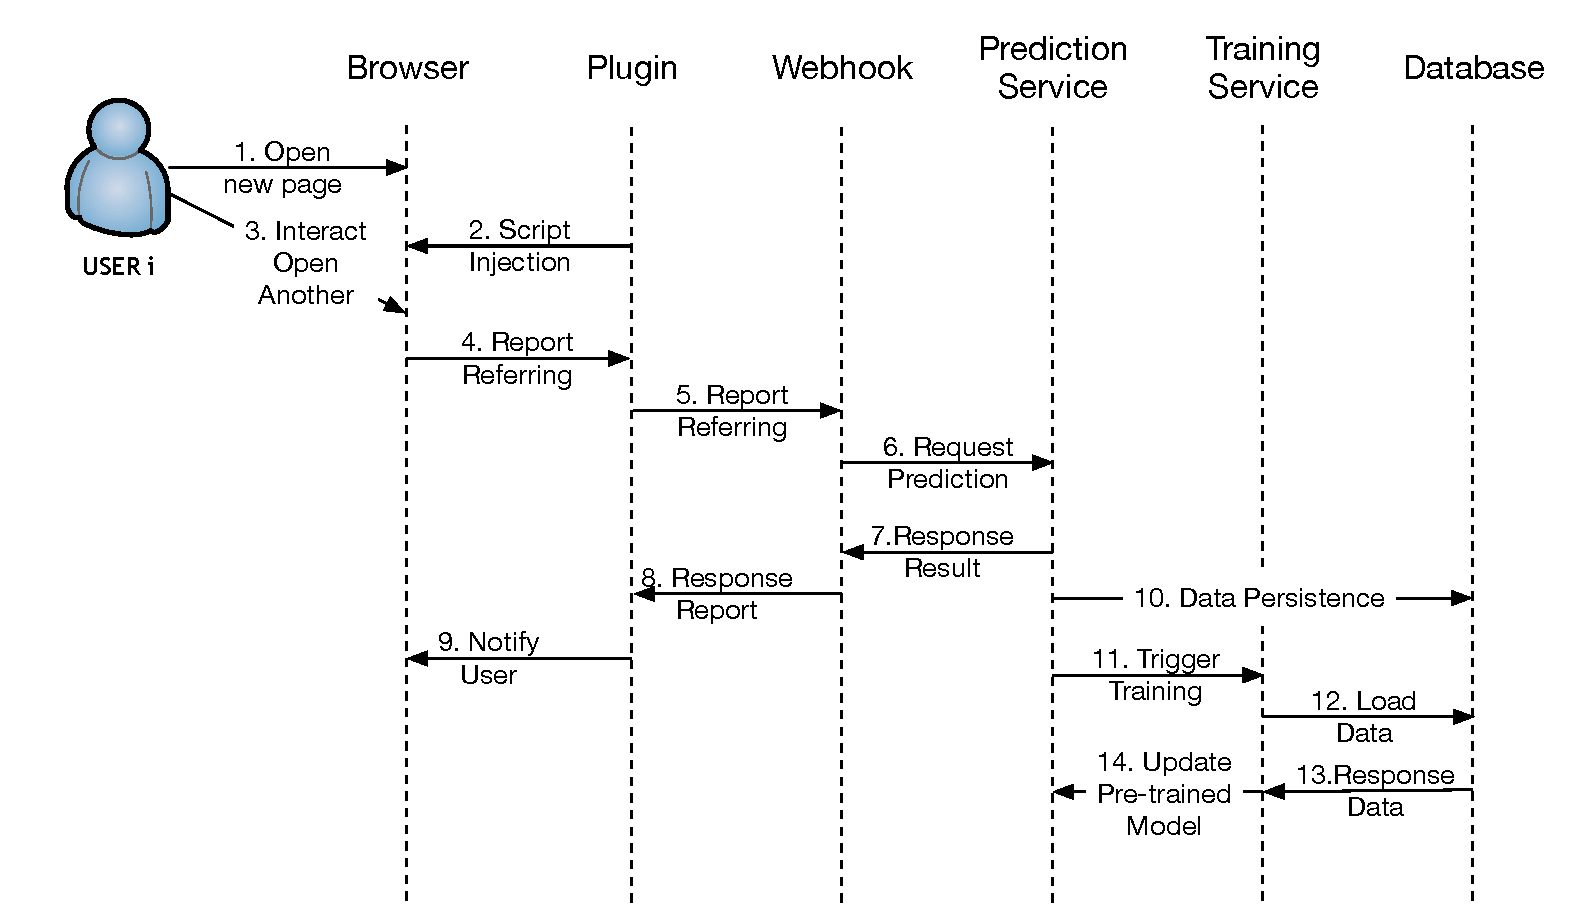
\includegraphics[width=0.7\textwidth]{figures/arch}
    \caption{TODO:}
    \label{fig:arch}
\end{figure}

\subsection{Web API Standardization and Platform-as-a-Service}

Web APIs is a generic term used in various fields of development.
Web APIs in a context of web browsers mainly indicates the APIs provided
by browser manufactures to developers that helps web application can even close
to manipulate hardwares, for instance, WebAssembly \cite{w3c2018ws}.

Nowadays, there are experimental standard Web APIs integrates complex features to 
web developers, e.g. Web Speech APIs \cite{mozilla2019speech}, and 
only Google Chrome (after version 24) support. 
The specification proposal was initiated by Google, according to 
the source code of Chromium Kernel, the APIs are implemented based on 
the speech recognition service provided 
by Google Cloud Platform 
\footnote{\url{https://github.com/chromium/chromium/blob/83928864c18362a4b0f84bad9bee4104f4655430/content/browser/speech/speech\_recognition\_engine.cc\#L35}, last accessed on January 03, 2019},
which provides us a signal that browser APIs does not only giving interfaces to
the hardware, but also access cloud platform services, i.e. Platform-as-a-Service integrated 
APIs.

The plugin we illustrated in Section \ref{sec:plugin} can also be integrated as a PaaS API
that embedded into web browsers, which simplifies the infrastructure of the plugin. 
As a developer, one can simply call the standardized API to report current user actions
then get a response of current behavior status and the prediction of future movement or 
actions, as the diagram shown in Figure \ref{fig:webapi}.

\begin{figure}[H]
    \centering
    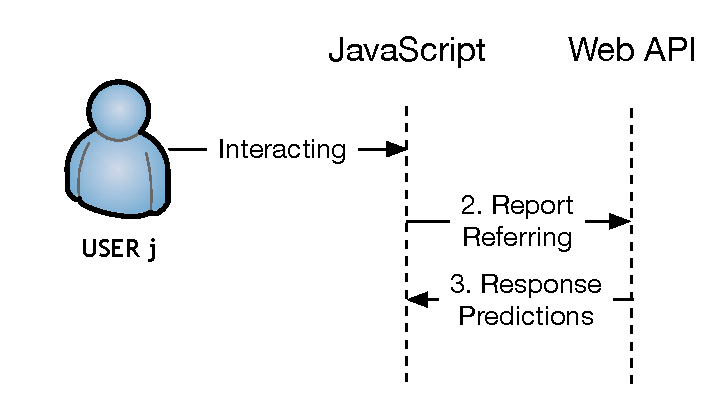
\includegraphics[width=0.4\textwidth]{figures/webapi}
    \caption{TODO:}
    \label{fig:webapi}
\end{figure}

Defining the specification of the Paas API aims enable web developers to
monitoring, in a web browser, the future actions of their user.
Developers can use the predicted actions to dynamically change the UI elements then improve
the user experience of their product. To keep the API to a minimum, we breifly discuss the
non-normative design of the browsing behavior predictor web API.

\subsubsection{The \emph{BrowsingBehavior} Interface}

The browsing behavior interface is the scripted web API for resulting a monitored browsing
session, which is presented in Code \ref{lst:interface}.

\begin{lstlisting}[
    language={JavaScript},
    caption={BrowsingBehavior Interface},
    label={lst:interface}
]
[Exposed=Window, Constructor]
interface BrowsingBehavior : EventTarget {
    
    // methods to drive browsing behavior response
    void start();
    void stop();
    void pause();
    void resume();

    // event methods
    attribute EventHandler onBrowsingStart;
    attribute EventHandler onBrowsingEnd;
    attribute EventHandler onBrowsingPause;
    attribute EventHandler onBrowsingResume;
    attribute EventHandler onResult;
}
\end{lstlisting}

\paragraph{\emph{start()} method} When start method is called, it represents the moment in
time the web application wishes to begin monitoring user's actions.
Then every step when user making actions, the \emph{EventHandler onResult} will produce
a standard prediction and classification of user browsing behavior. Further, 
the \emph{EventHandler onBrowsingStart} will be called immediatelly after calling 
this method and before resulting a prediction result, which gives a barrier in between of
calling \emph{start} and callback \emph{onResult}.

\paragraph{\emph{stop()} method} When stop method is called, it represents the instruction
to browsing behavior service to stop monitoring user actions, and resulting a final 
prediction in the \emph{EventHandler onBrowsingEnd}.

\paragraph{\emph{pause()} method} This method is used to ignoring the upcoming user actions
to pauses the monitoring of user actions, and resulting a prediction in the 
\emph{EventHandler onBrowsingPause}.

\paragraph{\emph{resume()} method} This method resumes the paused \emph{BrowsingBehavior}
object and recover the monitoring of user actions. Before monitoring is fully recovered,
the \emph{EventHandler onBrowsingResume} will be called.

The major consideration of designing these four methods is to restrict an abuse of the APIs.
Similar to cookie, speech recognition APIs, a website should acquire an authorization from
their user, otherwise the API cannot monitor any user actions on the web, which partially
solves the issue of privacy and security. We will discuss more concerns of the feature in
Chapter \ref{ch:discuss}.

\subsubsection{\emph{onResult} callback}

\emph{onResult} callback passes the prediction after the browser user performed an action.
The prediction result consist two parts: behavior and future movements.

The \emph{behavior} attribute of the result object is a JSON object that contains 
confidence level, i.e. classification probability, and a enumerate \emph{category} attribute
that indicate the a finite set of user browsing behaviors, i.e. goal-oriented, fuzzy or exploring.

\begin{lstlisting}[
    language={JavaScript},
    caption={Result object of onResult callback},
    label={lst:callback}
]
{
    "behavior": {
        "confidence": float64,
        "category": string,
    },
    "futures": [
        {
            "confidence": float64,
            "actions": array[string],
        },
        {
            "confidence": float64,
            "actions": array[string],
        },
        ...
    ]
}
\end{lstlisting}

The \emph{futures} attribute of the result object is an ordered JSON object that from the
highest \emph{confidence} to lowerest {confidence} and the \emph{confidence} is a floating
number from minimum 0 to maximum 1 value. Meanwhile, the \emph{actions} attribute in a 
JSON object of an item of \emph{futures} array is an array of possible actions of URLs that
ordered in chronologic order, the first element represents the next immediate action,
and the last element represents the final action in the session, as shown in Code \ref{lst:callback}.

\begin{lstlisting}[
    language={JavaScript},
    caption={Formation of browser collections},
    label={lst:collect}
]
{
    "device_id": string,
    "previous_url": string,
    "current_url": string,
    "stay_seconds": float64,
    "time": string
}
\end{lstlisting}

From the perspective of implementation, browser manufactures collect data after developer
calls \emph{start()}.
In Code \ref{lst:collect}, each time when user performs an action, including open a new page,
switch to another tab or backtrack to former page, will result an JSON object that contains
\emph{device\_id} a unique identifier that represents the device, \emph{previous\_url} the previous
URL of the action, \emph{current\_url} the current URL of the action, \emph{stay\_seconds}
the stay duration of \emph{previous\_url} and \emph{time} string of the time of data creation.

% \subsubsection{Communication Protocol}

\cleardoublepage